
% www.brianrhall.net

% Document settings
\documentclass[11pt]{article}
\usepackage[margin=1in]{geometry}
\usepackage[pdftex]{graphicx}
\usepackage{multirow}
\usepackage{setspace}
\usepackage{listings}
\pagestyle{plain}
\setlength\parindent{0pt}

\begin{document}
	
	\section*{La machine frigorifique, la pompe à chaleur}
	
	Rappel (cours précédent) :  
	
	\subsection*{La machine frigorifique réversible}
	
	La machine thermique :
	
	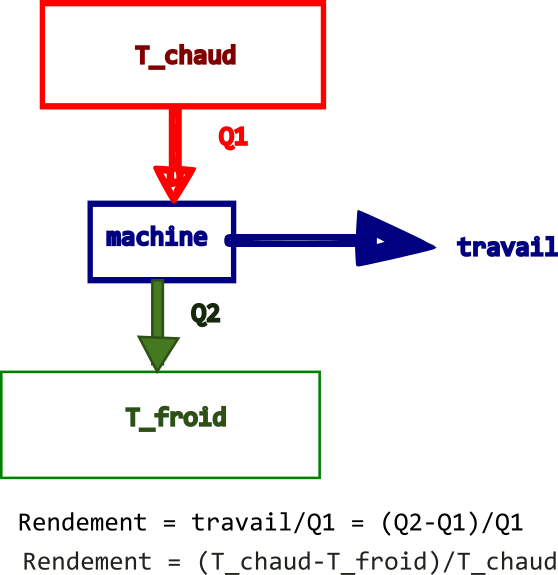
\includegraphics[width=0.7\linewidth]{images/machine_thermique.png}
	
	...
	
	La machine thermique peut être inversée : c’est le principe du réfrigérateur et de la pompe à chaleur.
	
	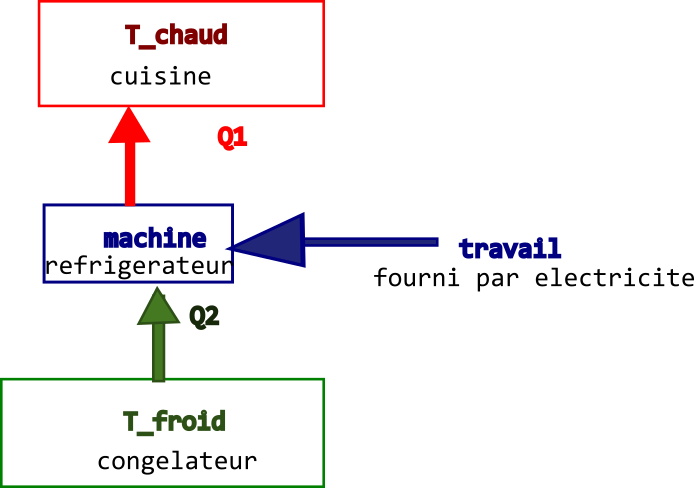
\includegraphics[width=0.7\linewidth]{images/machine_thermique_inv.png}
	
	C’est le principe de fonctionnement du réfrigérateur et de la pompe à chaleur.  
	La différence entre ces deux machines est que, dans le réfrigérateur, on utilise le refroidissement de la source froide, tandis que dans la pompe à chaleur, on exploite le réchauffement de la source chaude.  
	Dans les deux cas, un travail mécanique est fourni par un moteur électrique.
	
	\subsection*{La machine frigorifique réelle}
	
	La machine réversible nécessite de hautes pressions pour être efficace, ce qui est difficilement réalisable en pratique.  
	
	La machine frigorifique réelle utilise un fluide avec changement d’état liquide-gaz afin de tirer parti de la chaleur latente de changement d’état.  
	
	La chaleur est absorbée lorsque le liquide s’évapore.  
	Cependant, pour que la machine fonctionne en cycle, il faut comprimer puis condenser la vapeur, ce qui libère de la chaleur.  
	
	Avant d’étudier cette machine en détail, on doit remarquer qu’il existe deux grandes classes de machines thermiques :
	\begin{itemize}
		\item Machines à piston (dont le cycle de Carnot)
		\item Machines à écoulement, avec un écoulement continu de fluide dans la machine. Ce dernier type n’est pas étudié dans le cours de thermodynamique classique et relève de la thermodynamique industrielle.
	\end{itemize}
	
	\subsubsection{Système à écoulement : détendeur}
	Considérons un système isolé thermiquement.
	
	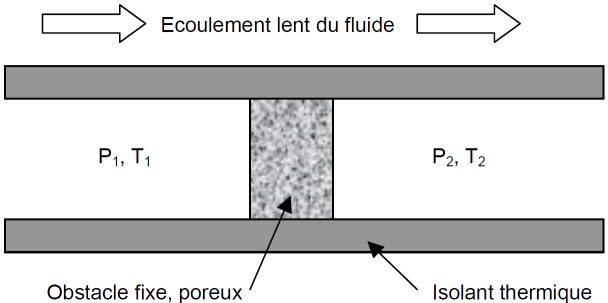
\includegraphics[width=0.7\linewidth]{images/exp_joule_thomson.png}
	
	La pression du gaz diminue pendant son passage de gauche à droite. Si l’on considère un volume de gaz $V_1$ sous la pression $P_1$ à gauche, alors à droite, sous la pression $P_2$, son volume devient $V_2$.  
	
	Sur cette quantité de gaz, le travail $W_1 = P_1 \times V_1$ est effectué par la portion de gaz suivante sous la pression $P_1$. Cette portion effectue le travail $W_2 = P_2 \times V_2$ sur la portion suivante (à droite).  
	
	La variation d’énergie interne est due exclusivement au travail en l’absence d’échange thermique :
	\[
	U_1 + W_1 - W_2 = U_2
	\]
	
	ou :
	\[
	H_1 = H_2 \quad \texttt{(on rappelle que } H = U + PV\texttt{)}
	\]
	
	La détente est donc isenthalpique.
	
	\subsubsection*{Système à écoulement : condenseur ou évaporateur}
	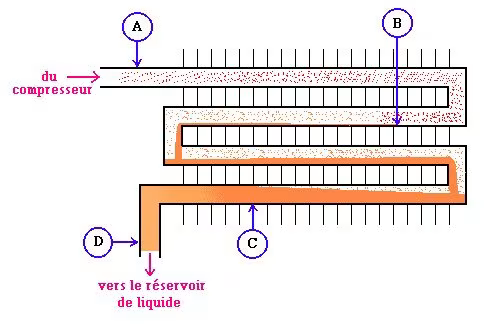
\includegraphics[width=0.7\linewidth]{images/condenseur fonctionnement.png}
	
	\begin{itemize}
		\item A : le gaz
		\item B : le mélange gaz + liquide
		\item C : le liquide + un peu de gaz
		\item D : le liquide
	\end{itemize}
	
	Ce processus est isobare avec émission de chaleur. L’évaporation se produit en sens inverse avec absorption de chaleur. 
	
	\subsubsection*{Schéma et fonctionnement de la machine frigorifique}	 
	
	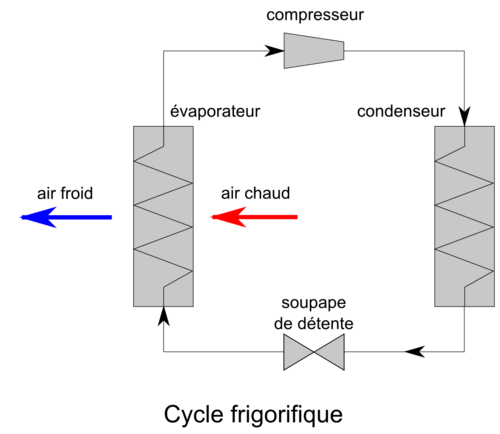
\includegraphics[width=0.7\linewidth]{images/machine_frigo.png}
	
	Nous avons maintenant tous les éléments de cette machine :
	
	\begin{itemize}
		\item A-B \textbf{Sans échange de chaleur} : le travail est fourni au compresseur ; la compression se fait sans échange de chaleur (adiabatiquement).
		
		\item B-D \textbf{La chaleur est émise} dans le condenseur (action recherchée dans la pompe à chaleur) : le gaz se liquéfie (passage à un mélange liquide-gaz). L'enthalpie du fluide diminue.
		
		\item D-E \textbf{Sans échange de chaleur} : dans la soupape de détente, la pression du fluide diminue (passage par une valve), ce qui facilite son évaporation. Il n’y a ni échange de chaleur ni travail lors de cette étape.
		
		\item E-A \textbf{La chaleur est absorbée} (action recherchée dans la machine frigorifique) dans l’évaporateur à pression constante. L'enthalpie du fluide augmente.
	\end{itemize}
	
	Le fonctionnement de cette machine est étudié sur le diagramme pression-enthalpie :
	
	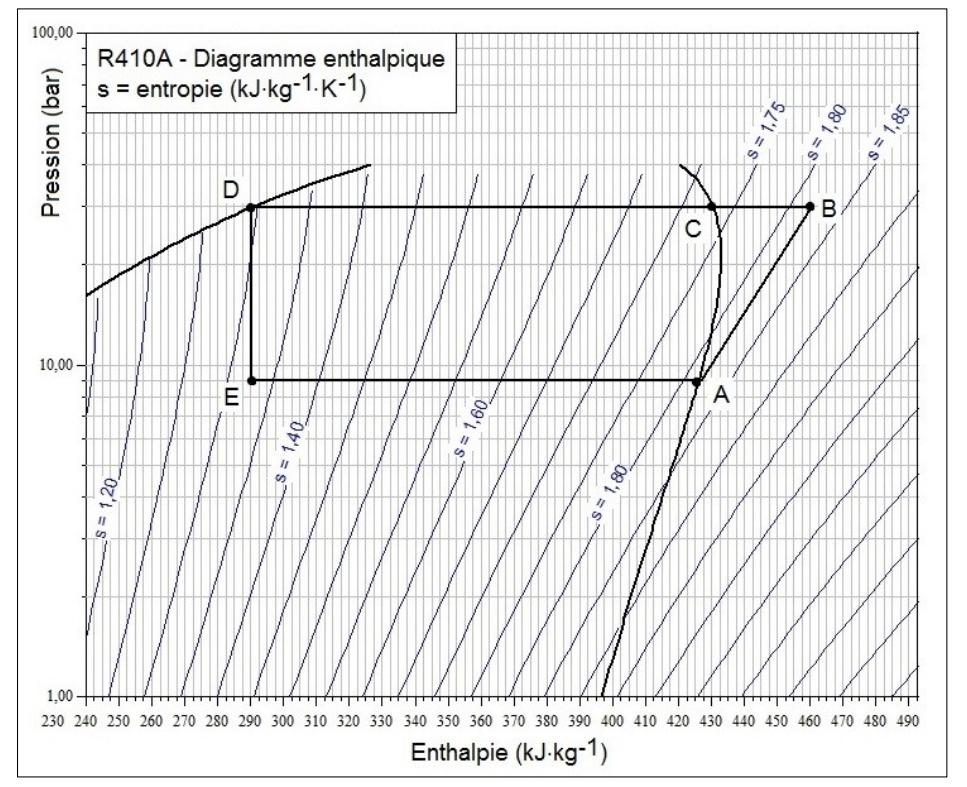
\includegraphics[width=0.7\linewidth]{images/hp_pompe.jpg}
	

\end{document}